\chapter{能量与哈密顿量}

\lectureoverview{我们首先厘清主动对称性的含义，并回顾平移与旋转如何生成动量和角动量。缺失的守恒定律是能量。它的对称性是时间平移，其守恒量是哈密顿量\(H=\sum_i p_i\dot q_i-L\)。这一推导还精确地表明，显式时间依赖如何在一个选定的子系统与其环境之间传递能量。}

\section{正式论证之前的问题}

我们正在接近后续主题所需的经典力学绝对最低限度，尽管仍有更多力学值得学习。在主要论证开始之前，出现了两个问题。

\begin{classroomqa}
  \audiencequestion{在这门入门课程之后，哪些书有用？
  \lecturetimestamp{00:00:36--00:02:13}}
  \lecturerresponse{公认的高级参考书是 Herbert
  Goldstein 的 \emph{Classical Mechanics}。Cornelius Lanczos 关于力学变分原理的书是另一个相关来源。一份班级阅读书单比假装一位讲师能够综述所有可用的教材更有用。}
\end{classroomqa}

第二个问题记录了历史上一个尚未解决的测量中的一个时刻。在 2011 年，OPERA 实验曾报告，从 CERN 发送到 Gran Sasso 的中微子似乎提前到达。所报告的差异比用于产生中微子的质子脉冲更短，因此时间分析依赖于比较脉冲轮廓，而不是在发射时标记一个中微子并在探测时识别同一个粒子。

\begin{classroomqa}
  \audiencequestion{那个表观超光速中微子结果是否已经解决？
  \lecturetimestamp{00:02:30--00:09:03}}
  \lecturerresponse{当时没有理由得出任何结论。束流脉冲形状、靶加热和同步都要求技术上的仔细审查。一个推测性提议考虑了 GPS 卫星的运动：在卫星参考系中，源和探测器在运动，而定时信号在传播，从而产生数十纳秒量级的修正。作为数量级练习，这个估计很有趣，但它并未被当作对该实验的可信诊断提出。在相关速度下，普通的洛伦兹收缩太小，无法提供所报告的效果。正确的回应是等待实验分析。}
\end{classroomqa}

\begin{figure}[htbp]
  \centering
  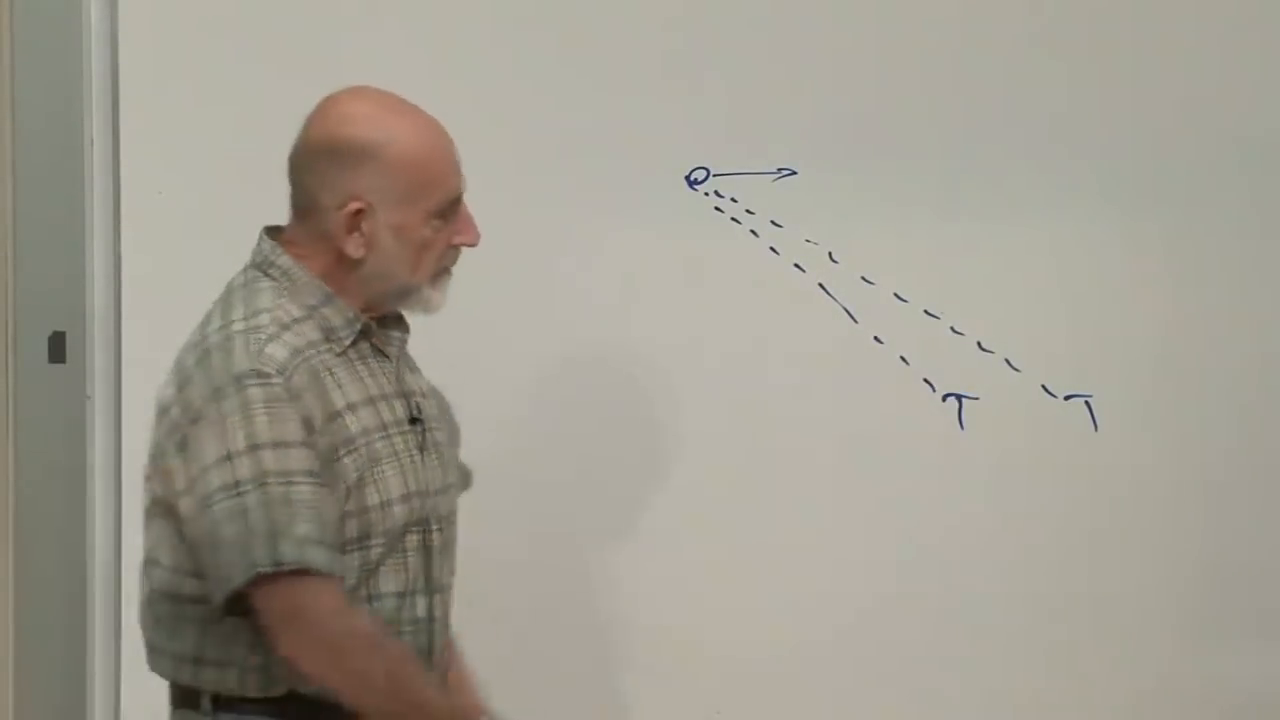
\includegraphics[width=0.78\textwidth]{lecture_05_figure_07.png}
  \caption{在历史性中微子测量问题期间讨论的卫星参考系定时草图。}
  \lectureframe{00:06:30}
\end{figure}

下面的力学不需要这段定时讨论。尽管如此，它仍然有用，因为它提醒我们，一个看似合理的尺度估计并不等同于一个已确立的实验解释。

\section{主动对称性与系统的选择}

让我们回到前面讨论中过于模糊的那一点：对称性究竟是什么？考虑一条直线上的一个粒子以及指令
\begin{equation}
  x\longrightarrow x+1.
  \label{eq:l5-shift-one}
\end{equation}
有两种理解方式。一个\emph{被动}变换重新标记直线上的点。一个曾被称为\(x=0\)的点现在可以被称为\(x'=1\)，但粒子并没有移动。一个\emph{主动}变换保持标签固定，并移动粒子本身，从\(x\)到\(x+1\)。只有第二种操作会改变它相对于外部势的位置。

\begin{figure}[htbp]
  \centering
  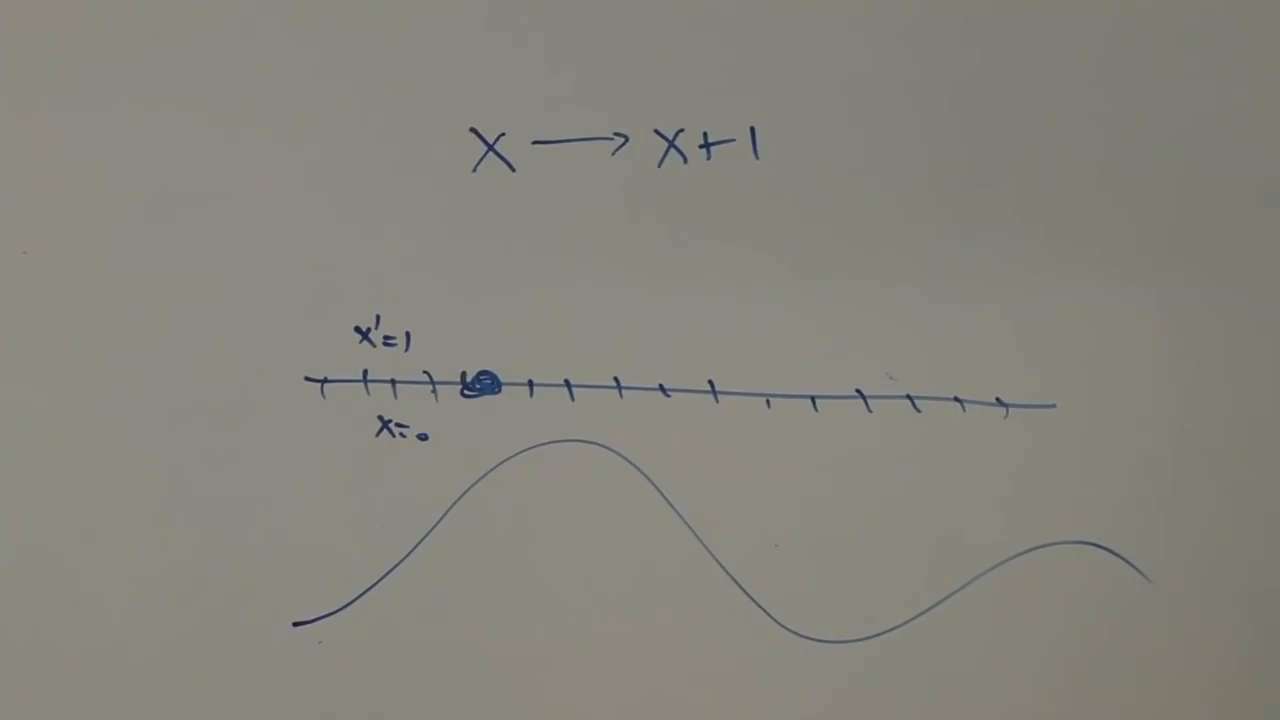
\includegraphics[width=0.82\textwidth]{lecture_05_figure_08.png}
  \caption{规则\(x\mapsto x+1\)、固定的坐标线以及一个外部势，将主动运动与被动重新标记区分开来。}
  \lectureframe{00:11:20}
\end{figure}

\begin{classroomqa}
  \audiencequestion{如果移动粒子会改变它的势能，那么该势的来源是否被排除在系统之外？
  \lecturetimestamp{00:12:19--00:14:18}}
  \lecturerresponse{正是如此。把系统称为``势中的粒子''，就是把世界划分为粒子与一个产生\(V(x)\)的重环境，例如地球。地球确实会反冲，但在这个近似中，其巨大的质量使这种反冲可以忽略不计。相对于固定地球移动粒子可以改变\(V\)；把粒子与地球一起平移则不会。}
\end{classroomqa}

\begin{classroomqa}
  \audiencequestion{在早先的旋转例子中，速度是否和位置一样也被改变了？
  \lecturetimestamp{00:14:26--00:15:29}}
  \lecturerresponse{是的。刚性主动旋转作用于整个历史，而不只是作用于某一个瞬时位置。位置和速度矢量都被旋转。相比之下，在每一时刻施加的恒定平移会改变\(x\)，但使\(\dot x\)保持不变。}
\end{classroomqa}

系统与环境之间的区分将再次出现两次：一次是含时装置与一个子系统交换能量时，另一次是宏观摩擦把能量隐藏在未被观测到的微观运动之中时。

\section{位形空间中的无穷小运动}

一般力学系统的位形是广义坐标\(q_i\)空间中的一个点。一个主动无穷小变换把每一个可能的位形移动到附近的一个位形。我们写出
\begin{equation}
  \delta q_i=\epsilon f_i(q),
  \label{eq:l5-general-transformation}
\end{equation}
其中函数\(f_i\)规定了位形空间上的一个固定位移场。它们可以依赖于所有坐标，其中一些也可以为零。公因子\(\epsilon\)很小；它把步长的大小与变换的形状分离开来。

\begin{figure}[htbp]
  \centering
  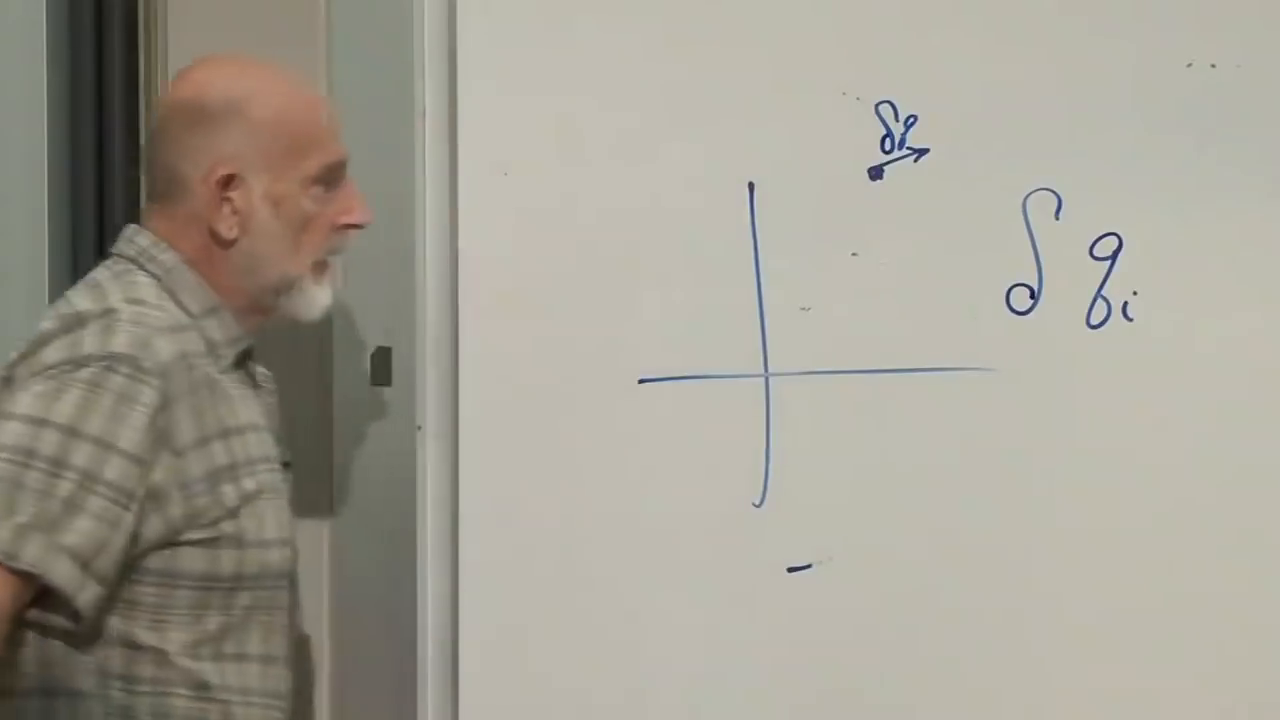
\includegraphics[width=0.75\textwidth]{lecture_05_figure_09.png}
  \caption{附着在位形空间每一点上的位移矢量。}
  \lectureframe{00:16:50}
\end{figure}

\begin{figure}[htbp]
  \centering
  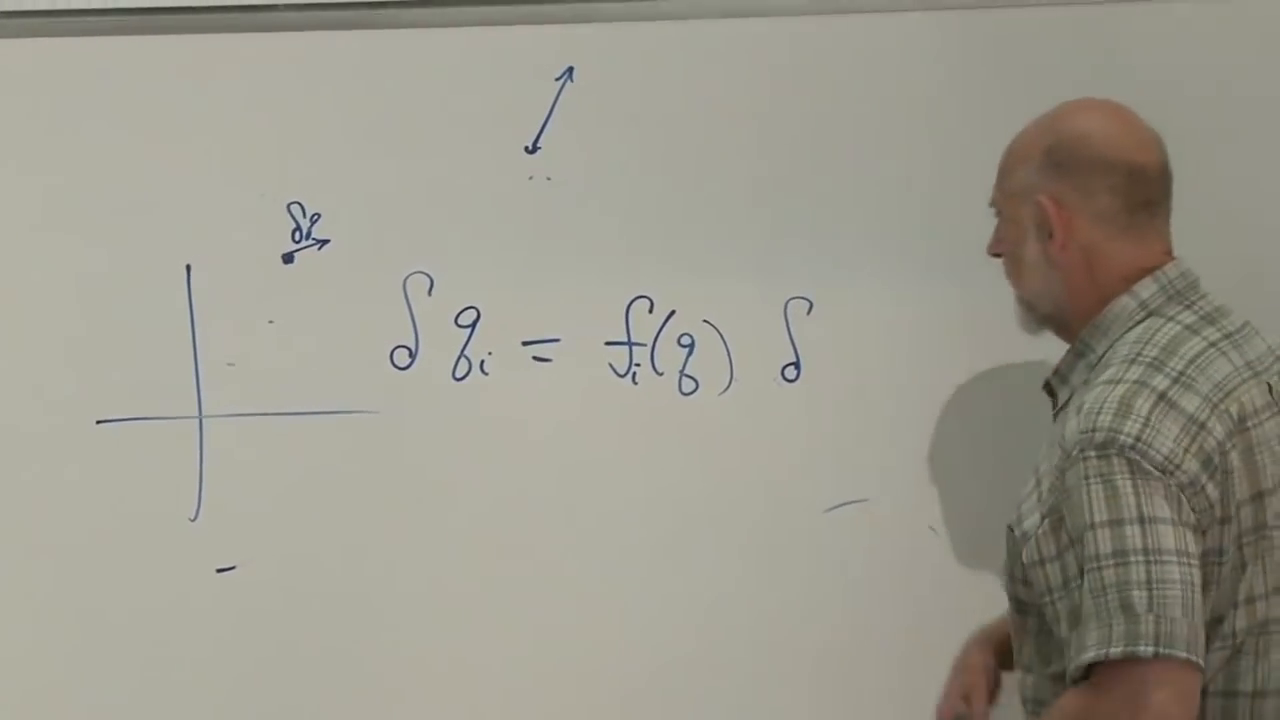
\includegraphics[width=0.80\textwidth]{lecture_05_figure_10.png}
  \caption{依赖于坐标的无穷小变换
  \(\delta q_i=\epsilon f_i(q)\)。}
  \lectureframe{00:18:00}
\end{figure}

该规则本身没有显式的时间依赖。因此它对速度的作用为
\begin{equation}
  \delta\dot q_i=\frac{d}{dt}(\delta q_i)
  =\epsilon\sum_j\frac{\partial f_i}{\partial q_j}\dot q_j.
  \label{eq:l5-velocity-variation}
\end{equation}
对于平移，\(f_x=1\)，所以\(\delta\dot x=0\)。对于旋转，\(f_i\)依赖于位置，速度会发生变化。

\begin{classroomqa}
  \audiencequestion{在
  \(\delta q_i=\epsilon f_i(q)\)中，最后那个小因子在每一点都是同一个常数吗？
  \lecturetimestamp{00:19:58--00:20:51}}
  \lecturerresponse{是的。这个单一的常数\(\epsilon\)是一种记账手段，它使所有坐标变化都是同一个微小量的一阶量。包含空间依赖的是函数\(f_i(q)\)，而不是\(\epsilon\)，并且它们本身不必很小。}
\end{classroomqa}

\section{是什么使变换成为对称性？}

主动变换一般会改变势能。它也可以改变动能。在曲线坐标中，动能项具有如下形式
\begin{equation}
  T=\frac12\sum_{i,j}g_{ij}(q)\dot q_i\dot q_j,
  \label{eq:l5-kinetic-metric}
\end{equation}
因此在位形空间中移动可以改变它的系数。极坐标中熟悉的\(r^2\dot\theta^2\)项就是最简单的例子。

在这里，当\emph{整个}拉格朗日量没有一阶变化时，该变换就是对称性，
\begin{equation}
  \delta L=O(\epsilon^2),
  \label{eq:l5-symmetry-condition}
\end{equation}
并且这必须在位形空间的每一点都成立，而不只是在某个特定解所占据的位形处成立。

例如，在\(x\mapsto x+\epsilon\)下，
\begin{equation}
  \delta V=\frac{\partial V}{\partial x}\epsilon.
  \label{eq:l5-potential-variation}
\end{equation}
如果这对每一个可能的\(x\)都为零，那么\(\partial V/\partial x=0\)：势能不依赖于\(x\)。如果它在沿每一个空间方向的平移下都不变，那么它就是常数。

\begin{figure}[htbp]
  \centering
  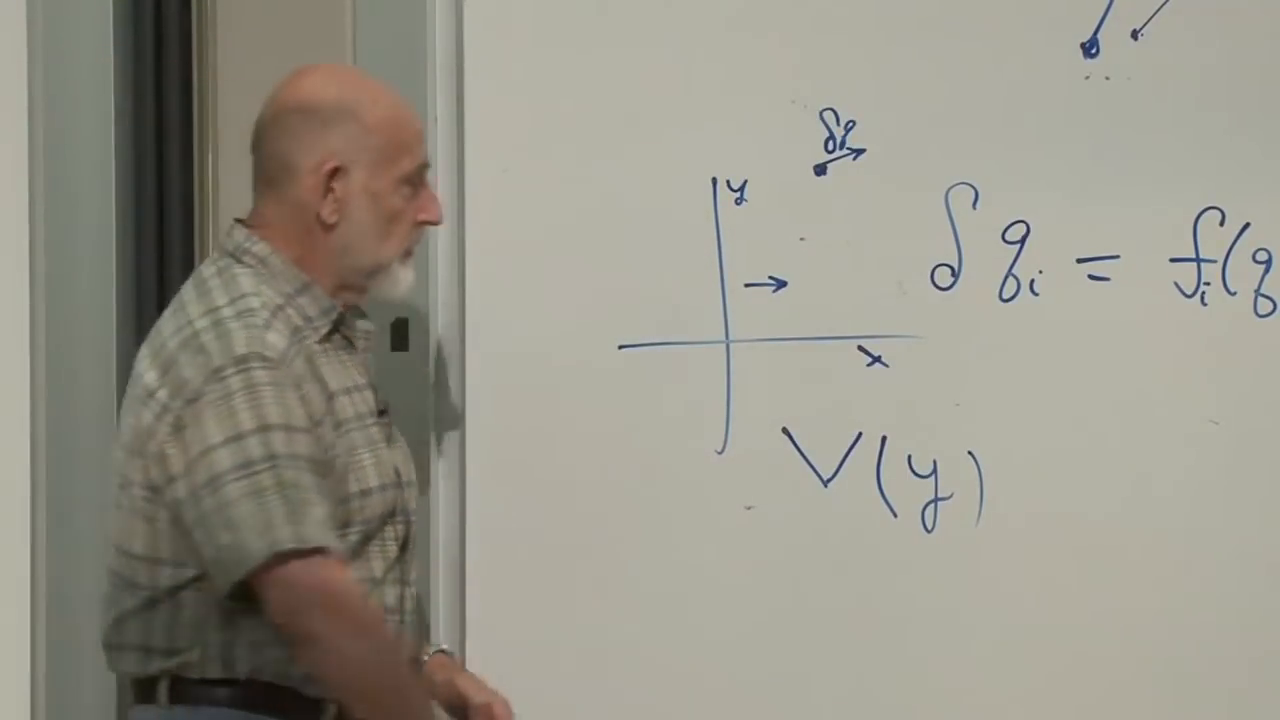
\includegraphics[width=0.80\textwidth]{lecture_05_figure_11.png}
  \caption{一个\(x\)平移，针对一个不依赖于\(V(y)\)的势能\(x\)进行检验。}
  \lectureframe{00:23:40}
\end{figure}

对于一个光滑的单参数族，每一点处一阶变化为零这一条件使我们能够把无穷小步骤复合为有限的对称性。

\begin{classroomqa}
  \audiencequestion{动能和势能必须分别保持不变吗？
  \lecturetimestamp{00:24:44--00:25:33}}
  \lecturerresponse{不。只有总拉格朗日量必须不变。有些拉格朗日量包含坐标--速度混合项，不允许有用地区分为\(T\)和\(V\)，因此分别不变甚至可能不是一个有意义的问题。}
\end{classroomqa}

\begin{classroomqa}
  \audiencequestion{``没有变化''是指确切地没有变化，还是仅仅指变化小到可以忽略？
  \lecturetimestamp{00:25:34--00:28:59}}
  \lecturerresponse{对于一个无穷小变换，它指的是没有正比于\(\epsilon\)的项。在局部计算中，\(\epsilon^2\)阶的项被丢弃。由于一阶条件沿单参数轨道处处成立，重复局部步骤就得到有限的对称性。}
\end{classroomqa}

\section{动量与角动量的重新得到}

对于这里所考虑的精确的、不含时的点对称性，先前证明的结果是
\begin{equation}
  Q=\sum_i p_i f_i(q),
  \qquad
  p_i=\frac{\partial L}{\partial\dot q_i},
  \qquad
  \dot Q=0.
  \label{eq:l5-noether-charge}
\end{equation}
因子\(\epsilon\)不属于\(Q\)；它只衡量我们沿对称性轨道移动了多远。

\begin{figure}[htbp]
  \centering
  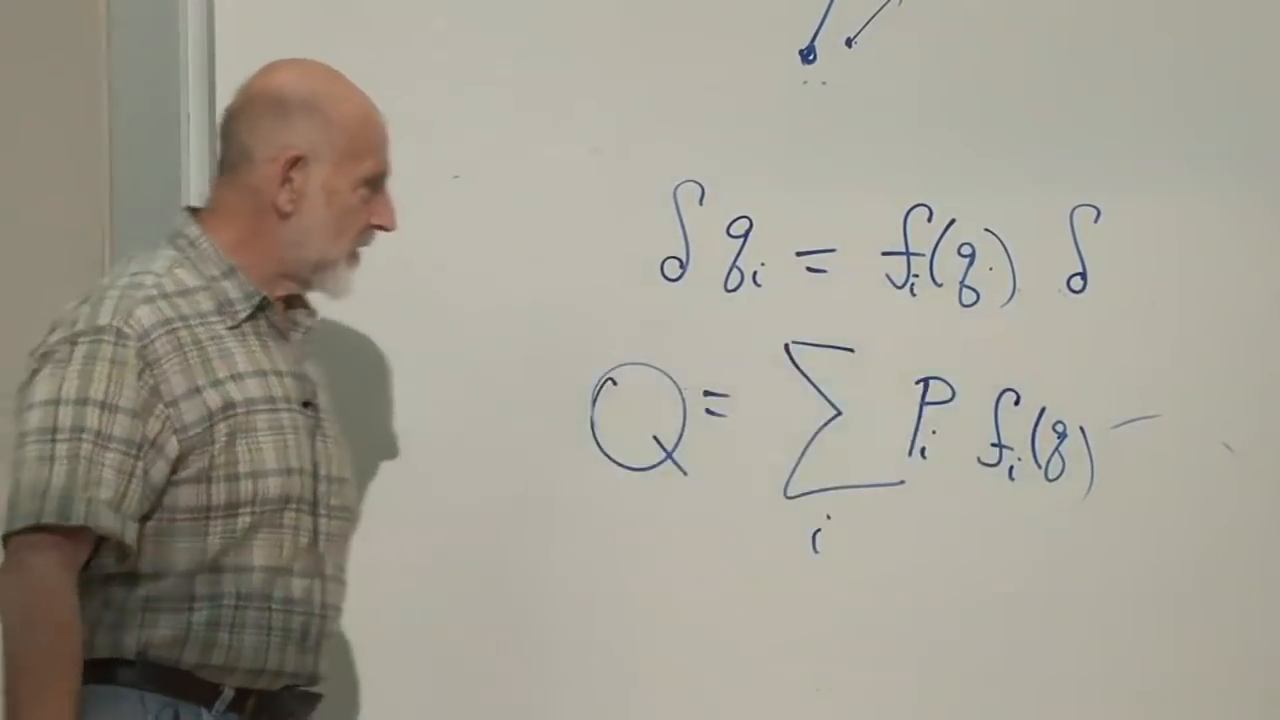
\includegraphics[width=0.82\textwidth]{lecture_05_figure_12.png}
  \caption{一般的无穷小位移及其守恒的诺特荷。}
  \lectureframe{00:30:00}
\end{figure}

对于沿\(x\)的平移，\(f_x=1\)，且\(Q=p_x\)。完全的平移不变性给出动量三个分量的守恒。对于许多相互作用的粒子，该对称性把每一个粒子一起平移，因此当相互作用只依赖于相对位置时，\begin{equation}
  \mathbf P=\sum_a\mathbf p_a
  \label{eq:l5-total-momentum}
\end{equation}守恒。让一个粒子相对于其余粒子移动并不是该对称性。

\begin{figure}[htbp]
  \centering
  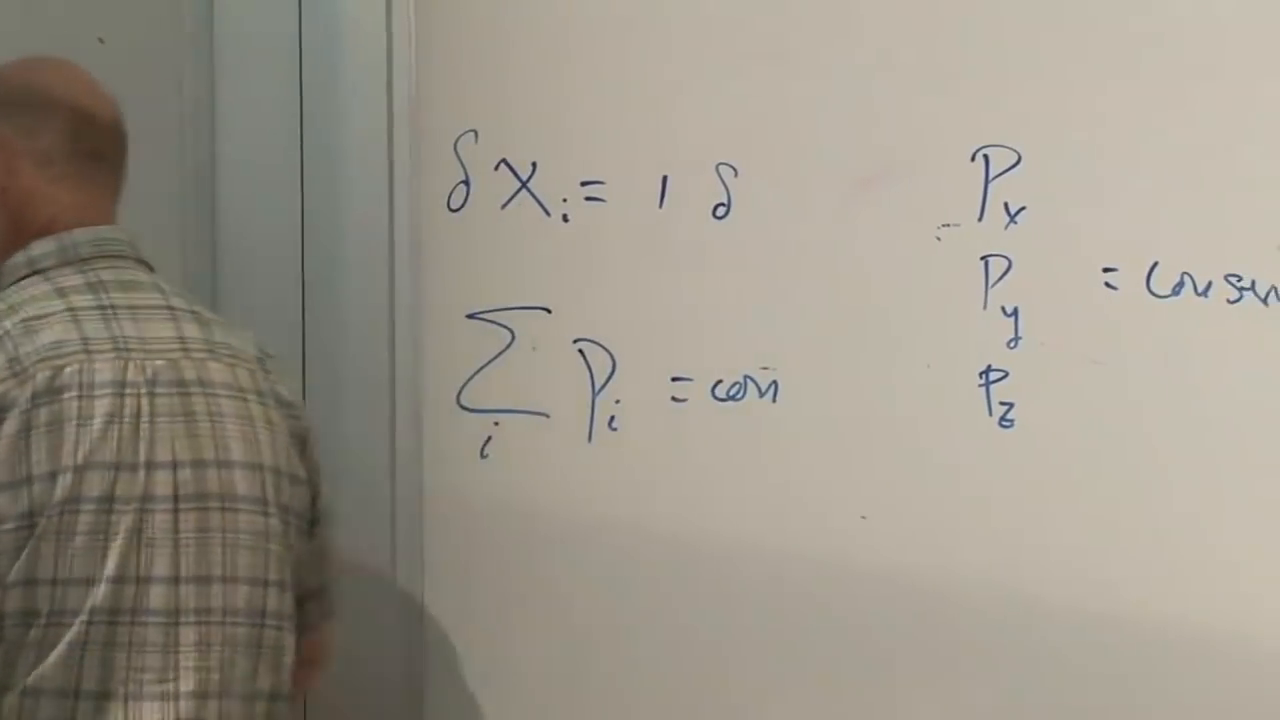
\includegraphics[width=0.80\textwidth]{lecture_05_figure_13.png}
  \caption{共同的平移产生总动量逐分量的守恒。}
  \lectureframe{00:32:50}
\end{figure}

对于\(x\)-\(y\)平面内的无穷小旋转，选择取向
\begin{equation}
  \delta x=-y\epsilon,
  \qquad
  \delta y=x\epsilon.
  \label{eq:l5-planar-rotation}
\end{equation}
它保持半径不变，因为
\begin{equation}
  \delta(x^2+y^2)
  =2x\delta x+2y\delta y=0.
  \label{eq:l5-radius-invariance}
\end{equation}

\begin{figure}[htbp]
  \centering
  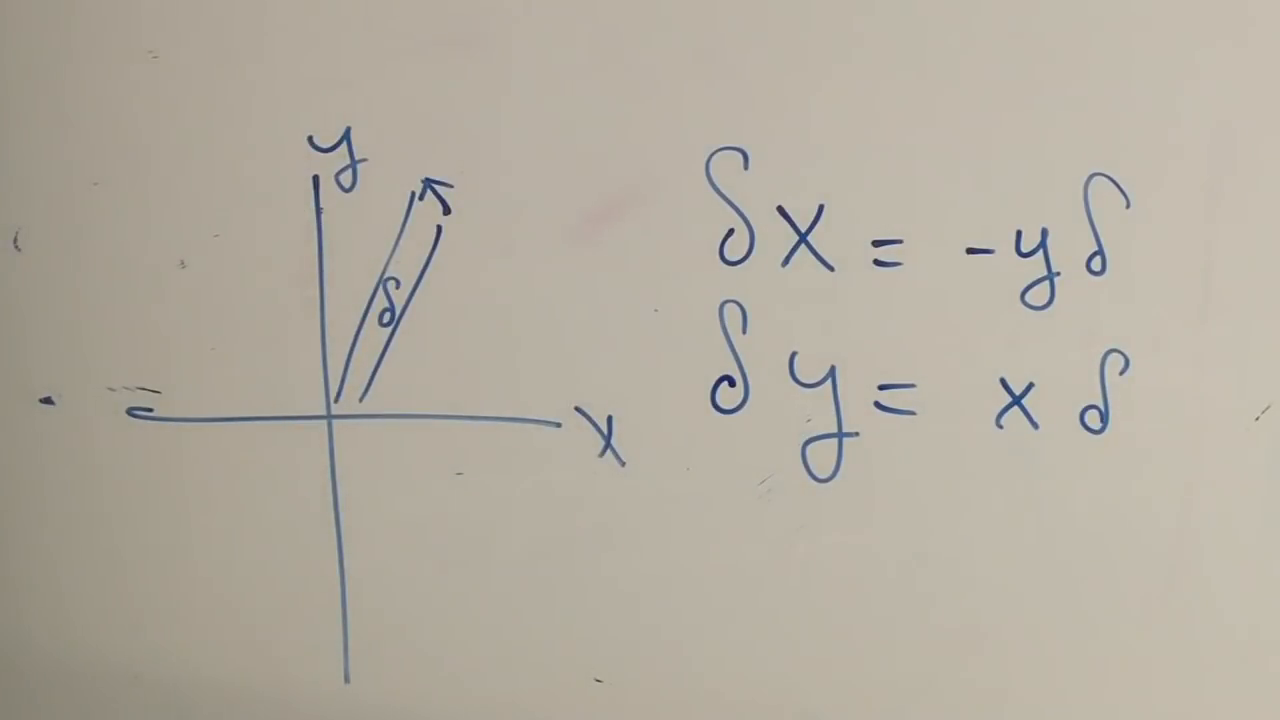
\includegraphics[width=0.76\textwidth]{lecture_05_figure_14.png}
  \caption{无穷小平面旋转的几何与坐标公式。}
  \lectureframe{00:35:05}
\end{figure}

对式~\eqref{eq:l5-planar-rotation}求导也会使速度发生同样的旋转。因此\(\dot x^2+\dot y^2\)是不变量，而中心势\(V(\sqrt{x^2+y^2})\)使整个拉格朗日量保持不变。该荷为
\begin{equation}
  Q=-yp_x+xp_y=(\mathbf r\times\mathbf p)_z.
  \label{eq:l5-angular-charge}
\end{equation}

\begin{figure}[htbp]
  \centering
  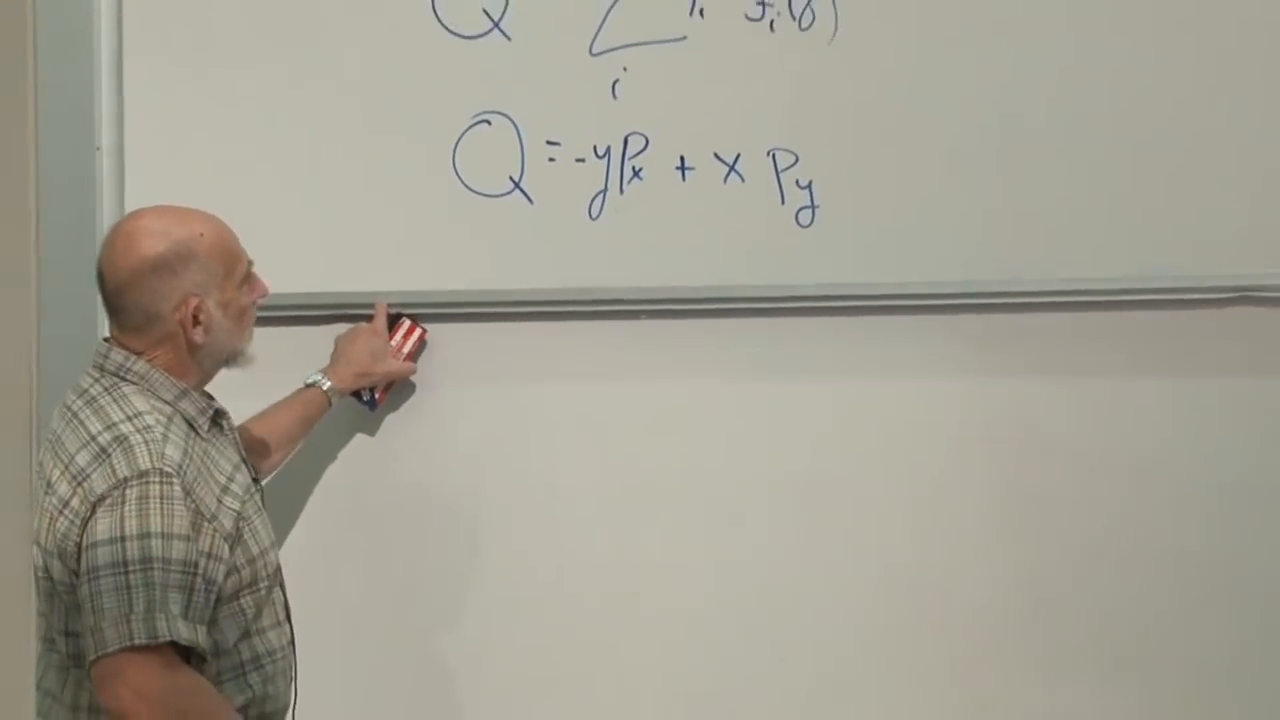
\includegraphics[width=0.76\textwidth]{lecture_05_figure_15.png}
  \caption{旋转诺特荷，即角动量的\(z\)分量。}
  \lectureframe{00:38:50}
\end{figure}

在其他坐标平面内的旋转给出其余分量。对于多粒子体系，守恒矢量是
\begin{equation}
  \mathbf J=\sum_a\mathbf r_a\times\mathbf p_a.
  \label{eq:l5-total-angular-momentum}
\end{equation}
中心恒星势中的行星是基本例子：在所有旋转下的不变性意味着角动量所有分量都守恒。

\begin{classroomqa}
  \audiencequestion{在尖锐的尖点处，一侧的导数与另一侧的导数不同，这时会怎样？
  \lecturetimestamp{00:42:25--00:44:21}}
  \lecturerresponse{这是一个合理的限定。目前的论证假定函数可微且导数唯一。不稳定平衡，例如物体在光滑极大值处保持平衡，本身并不是问题：该处的导数存在且为零。真正的尖点则需要修正的处理方式。}
\end{classroomqa}

\begin{classroomqa}
  \audiencequestion{如果变换参数与时间无关，为什么旋转会改变速度？
  \lecturetimestamp{00:44:23--00:45:23}}
  \lecturerresponse{参数是常数，但位移场依赖于坐标。普遍规则是
  \(\delta\dot q_i=d(\delta q_i)/dt\)。平移具有常数的
  \(\delta x\)，而旋转有\(\delta x=-y\epsilon\)，因此
  \(\delta\dot x=-\dot y\epsilon\)。}
\end{classroomqa}

\section{超出初等的动能减势能形式}

对于无磁场的普通非相对论粒子，在笛卡尔坐标下\(L=T-V\)。更一般的坐标给出式~\eqref{eq:l5-kinetic-metric}的二次型。磁场引入一个速度线性项，示意地写作\(\mathbf A(q)\cdot\dot{\mathbf q}\)，它把坐标与速度混合在一起。在这种情况下，最好把\(L(q,\dot q,t)\)当作一个函数来处理，而不是强行把每一项塞进传统的动能和势能框子里。

\begin{figure}[htbp]
  \centering
  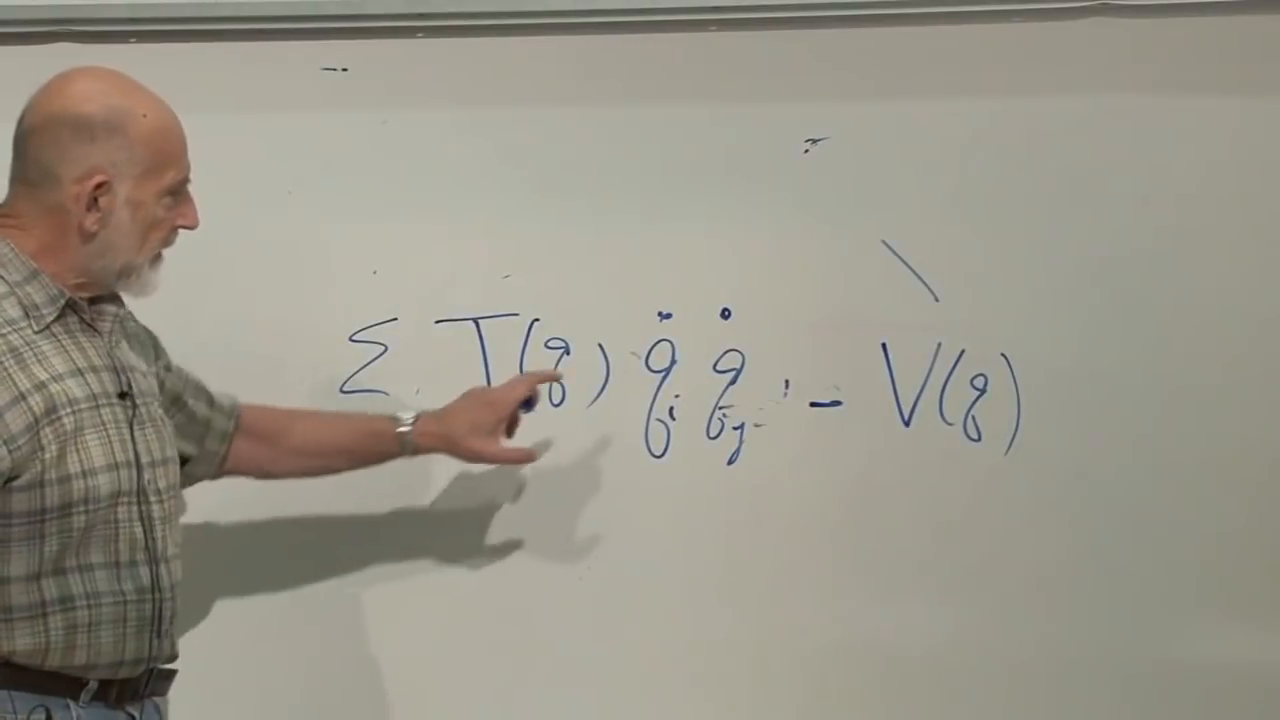
\includegraphics[width=0.80\textwidth]{lecture_05_figure_16.png}
  \caption{一般的依赖坐标的二次动能项与仅依赖坐标的势能项并列。}
  \lectureframe{00:47:20}
\end{figure}

\begin{classroomqa}
  \audiencequestion{为什么拉格朗日量可能无法干净地分离为动能和势能，它是否仍被定义为\(T-V\)？
  \lecturetimestamp{00:45:26--00:48:13}}
  \lecturerresponse{障碍可能来自曲线坐标，或来自诸如磁性这样的真正依赖速度的相互作用。只有当拉格朗日量由一个速度的二次型减去一个仅依赖坐标的函数组成时，我们才把那些部分命名为\(T\)和\(V\)。否则拉格朗日量仍然是\(q\)和\(\dot q\)的一个完全良好的函数，但这种拆分并无益处。能量的正确一般定义将来自哈密顿量。}
\end{classroomqa}

\begin{classroomqa}
  \audiencequestion{第一次课上讲的悬链例子是最小作用的应用吗？
  \lecturetimestamp{00:48:15--00:49:45}}
  \lecturerresponse{那是一个由最小能量支配的平衡问题，而不是由稳定作用选出的历史。对于普通\(T-V\)体系的静态解，\(\dot p_i=0\)，欧拉--拉格朗日方程化为\(\partial V/\partial q_i=0\)，即势能驻点的条件。}
\end{classroomqa}

动量与角动量现在都已与空间对称性联系起来。明显缺失的量是能量。

\section{时间平移不变性}

设想一个实验，它始于\(t_0\)，终于\(t_1\)，并产生一个结果。稍后重复同样的制备，始于
\(t_0+\Delta t\)，终于\(t_1+\Delta t\)。如果结果不变，则该系统在时间的主动平移下不变。

\begin{figure}[htbp]
  \centering
  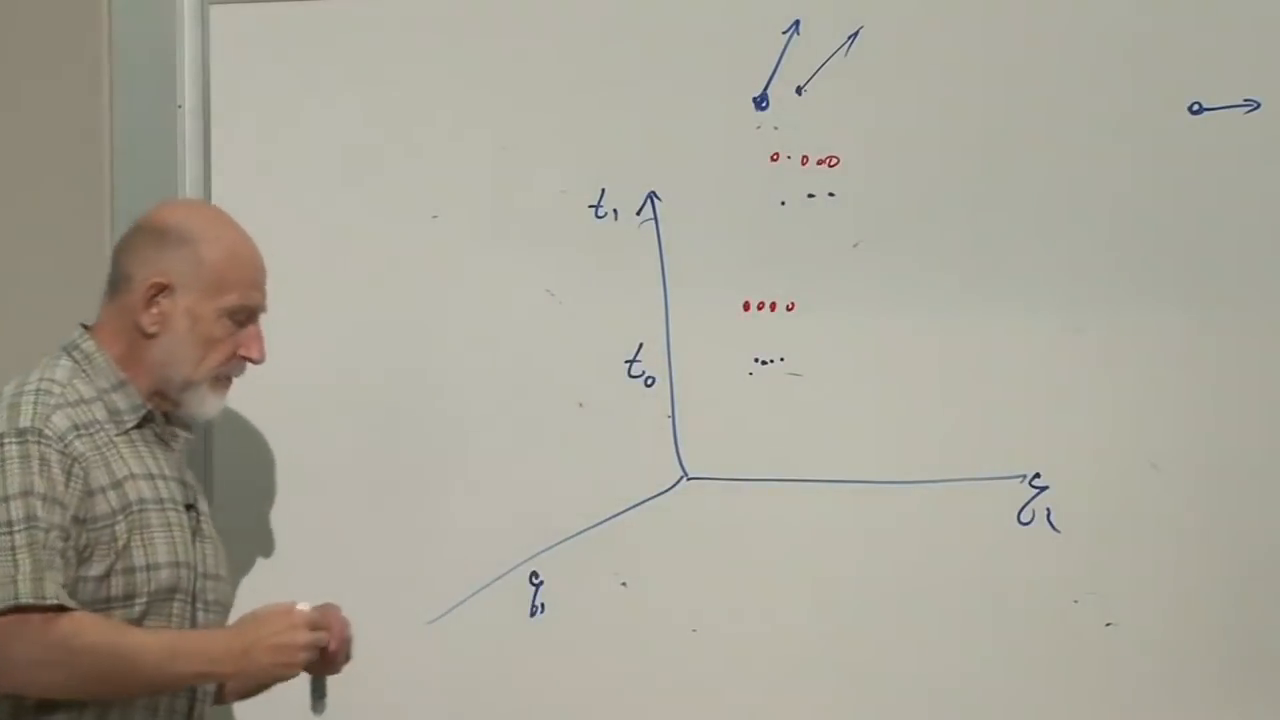
\includegraphics[width=0.82\textwidth]{lecture_05_figure_17.png}
  \caption{一个实验及其在位形空间历史中的时间平移副本。}
  \lectureframe{00:52:45}
\end{figure}

电容器极板之间的带电粒子说明了这一对称性的失效。在极板电荷固定的情况下，同一实验可以在任何时间进行。如果外部发电机正在稳定地给极板充电，那么粒子所感受到的电场取决于它何时被释放。此时粒子就是一个被显式驱动的子系统。

\begin{figure}[htbp]
  \centering
  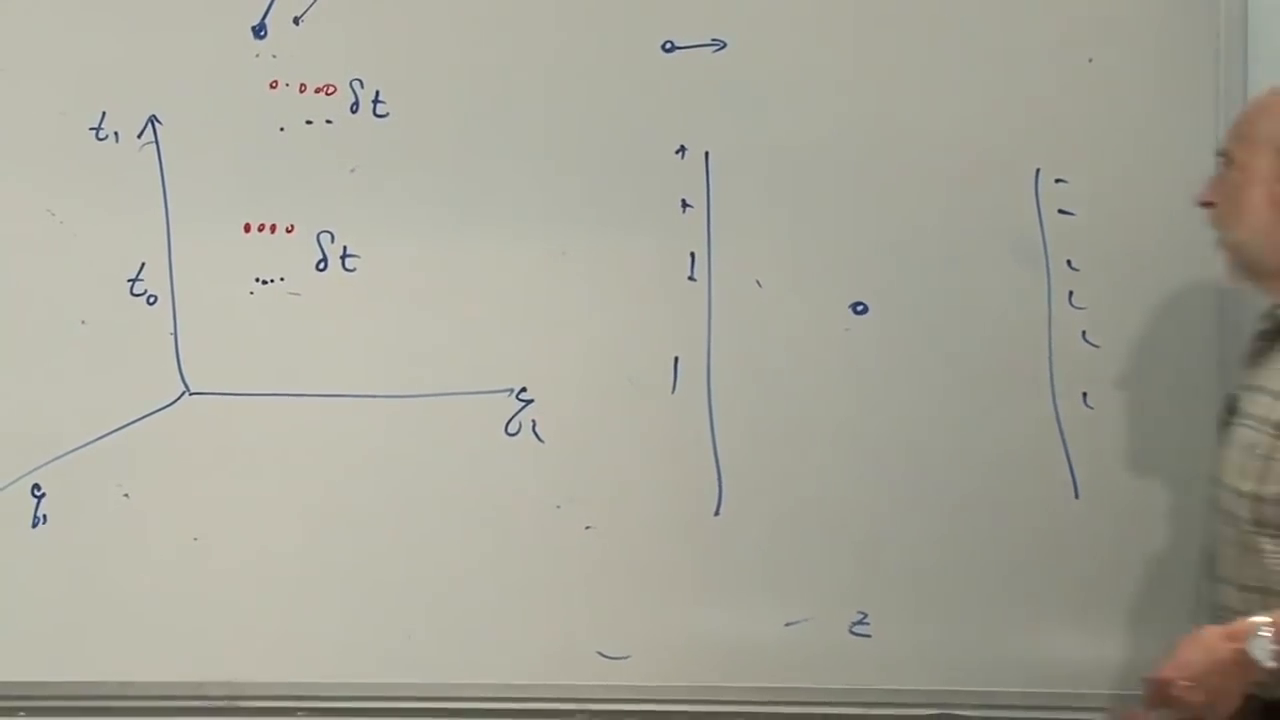
\includegraphics[width=0.82\textwidth]{lecture_05_figure_18.png}
  \caption{固定极板与外部变化的极板对比，旁边是时间平移示意图。}
  \lectureframe{00:54:45}
\end{figure}

同一点也出现在一个振子中，
\begin{equation}
  L=\frac12m\dot x^2-\frac12k(t)x^2.
  \label{eq:l5-driven-oscillator}
\end{equation}
外部电场或磁场可能会缓慢地改变材料，从而改变其有效弹簧常数。如果 \(k\) 变化，那么将振子实验在时间上平移就会改变结果。

\begin{figure}[htbp]
  \centering
  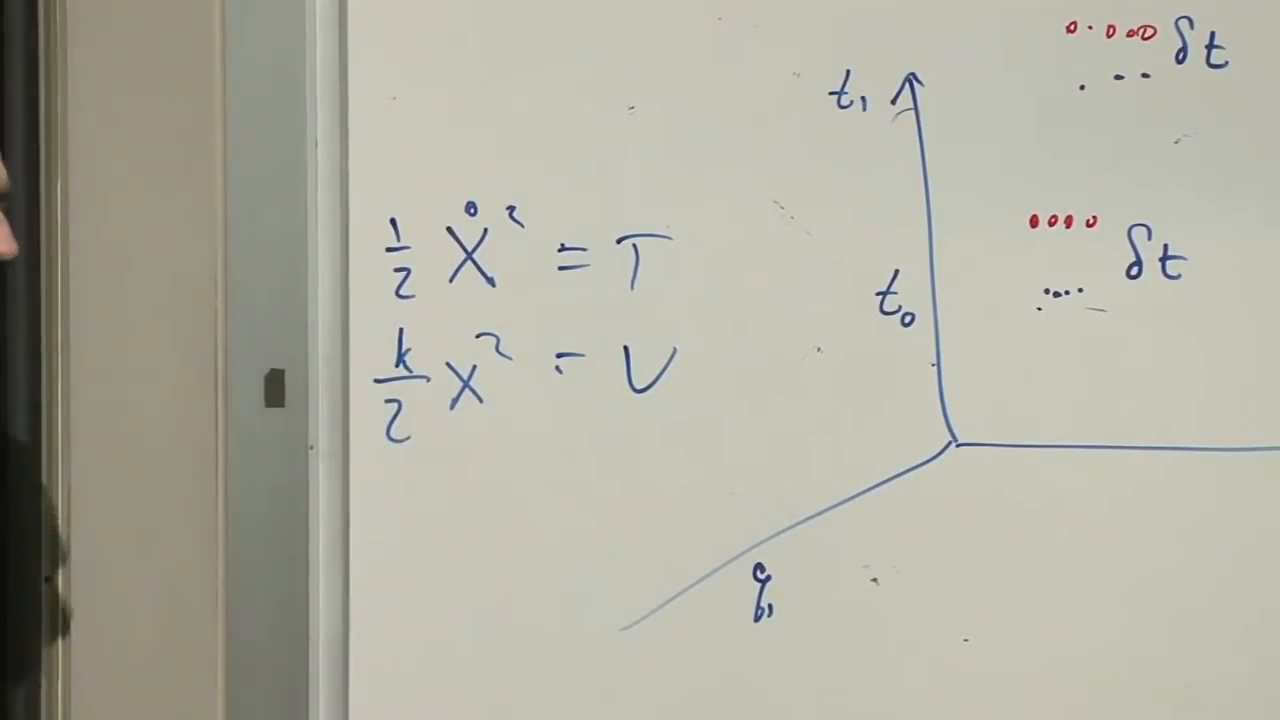
\includegraphics[width=0.78\textwidth]{lecture_05_figure_19.png}
  \caption{在讨论含时弹簧常数时振子的动能项和势能项。}
  \lectureframe{00:56:45}
\end{figure}

如果改变 \(k\) 的装置被包含在系统内，那么整个封闭实验又可以做时间平移，并且其总能量守恒。表面上的不守恒是能量跨越我们所选边界进行的交换。

在休息期间，小变换参数被重新命名为 \(\epsilon\)，以避免视觉上令人困惑的表达式 \(\delta x=\delta\)。关于一本讲述埃米·诺特的书的课堂推荐也被记入共享阅读清单。

\begin{classroomqa}
  \audiencequestion{如果拉格朗日量不是作为 \(T-V\) 给出的，那么它从哪里来？
  \lecturetimestamp{01:00:17--01:02:24}}
  \lecturerresponse{它可以从实验推断，由已知运动方程重构，根据对称性和其他理论原理猜测，或者通过试错找到。一旦 \(L(q,\dot q,t)\) 给定，欧拉--拉格朗日微积分就把它变成运动方程。形式论证并不要求我们先解决它的起源问题。}
\end{classroomqa}

时间平移不变性的操作检验现在很直接。如果知道 \(q\) 和 \(\dot q\) 就足以确定 \(L\)，而不还需要知道钟表时间，那么
\begin{equation}
  \frac{\partial L}{\partial t}=0.
  \label{eq:l5-no-explicit-time}
\end{equation}
这并不是说 \(L(q(t),\dot q(t))\) 沿运动是常数。它只是说，除了由演化中的坐标和速度所携带的时间依赖之外，不存在额外的时间依赖。

一个旋转的重哑铃提供了另一个受驱动例子。如果其规定运动为一个轻的检验粒子产生含时引力势，那么检验粒子的拉格朗日量就显含时间。若改为把哑铃动力学地处理，则会扩大系统并消除这种外部时间依赖。

\begin{figure}[htbp]
  \centering
  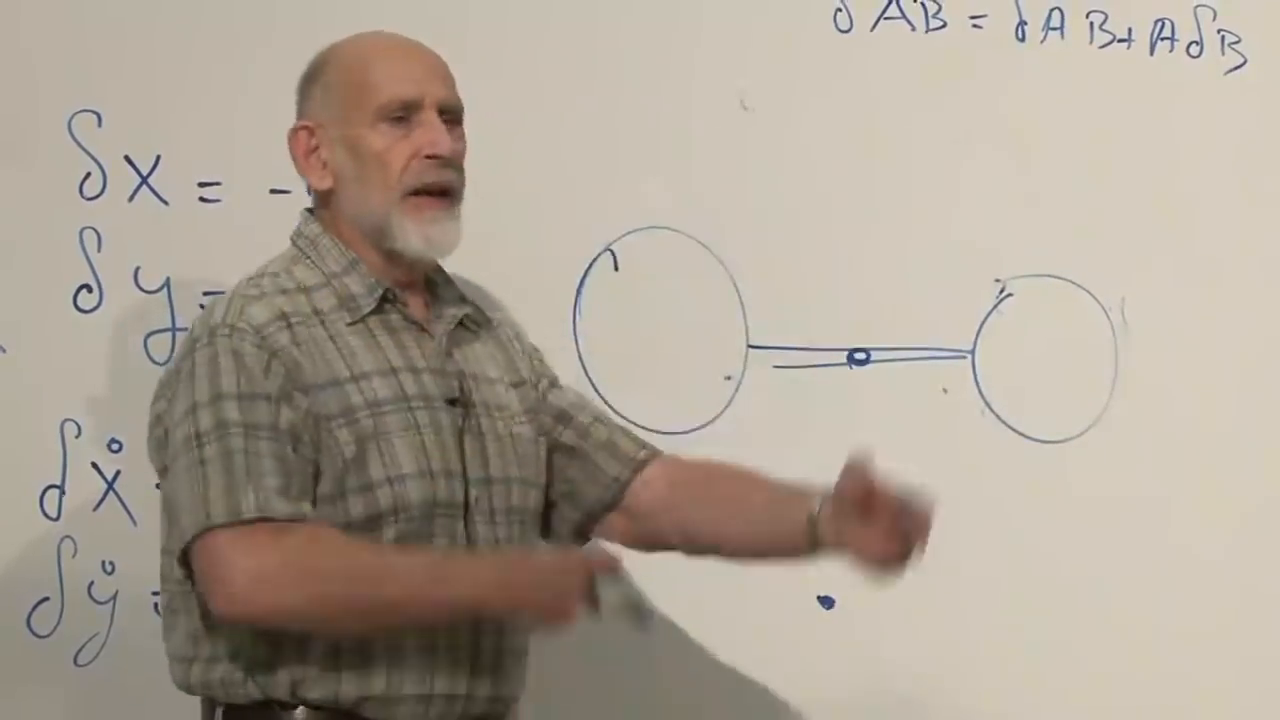
\includegraphics[width=0.80\textwidth]{lecture_05_figure_20.png}
  \caption{一个规定的旋转哑铃对较轻粒子充当含时外部源。}
  \lectureframe{01:06:25}
\end{figure}

\section{推导哈密顿量}

假设我们不知道能量的公式，并猜测也许拉格朗日量本身守恒。直接的检验是沿实际轨迹对它求导。为简单起见，先从没有显式时间依赖的情形开始：
\begin{equation}
  \frac{dL}{dt}
  =\sum_i\left(
    \frac{\partial L}{\partial q_i}\dot q_i
    +\frac{\partial L}{\partial\dot q_i}\ddot q_i
  \right).
  \label{eq:l5-chain-rule-no-time}
\end{equation}

\begin{figure}[htbp]
  \centering
  \includegraphics[width=0.72\textwidth]{lecture_05_figure_02.png}
  \caption{开始求 \(L(q_i,\dot q_i)\) 沿轨迹的导数。}
  \lectureframe{01:08:51}
\end{figure}

\begin{classroomqa}
  \audiencequestion{链式法则表达式中是否缺少一个求和？
  \lecturetimestamp{01:10:39--01:11:05}}
  \lecturerresponse{是的。每个坐标和每个速度都能改变拉格朗日量，所以两项都要对 \(i\) 求和。}
\end{classroomqa}

使用正则动量和欧拉--拉格朗日方程，
\begin{equation}
  p_i=\frac{\partial L}{\partial\dot q_i},
  \qquad
  \dot p_i=\frac{\partial L}{\partial q_i}.
  \label{eq:l5-p-and-pdot}
\end{equation}
于是式~\eqref{eq:l5-chain-rule-no-time}变为
\begin{align}
  \frac{dL}{dt}
  &=\sum_i(\dot p_i\dot q_i+p_i\ddot q_i)
  \notag\\
  &=\frac{d}{dt}\sum_i p_i\dot q_i.
  \label{eq:l5-product-rule}
\end{align}
这个``魔法''只是乘积法则。

\begin{figure}[htbp]
  \centering
  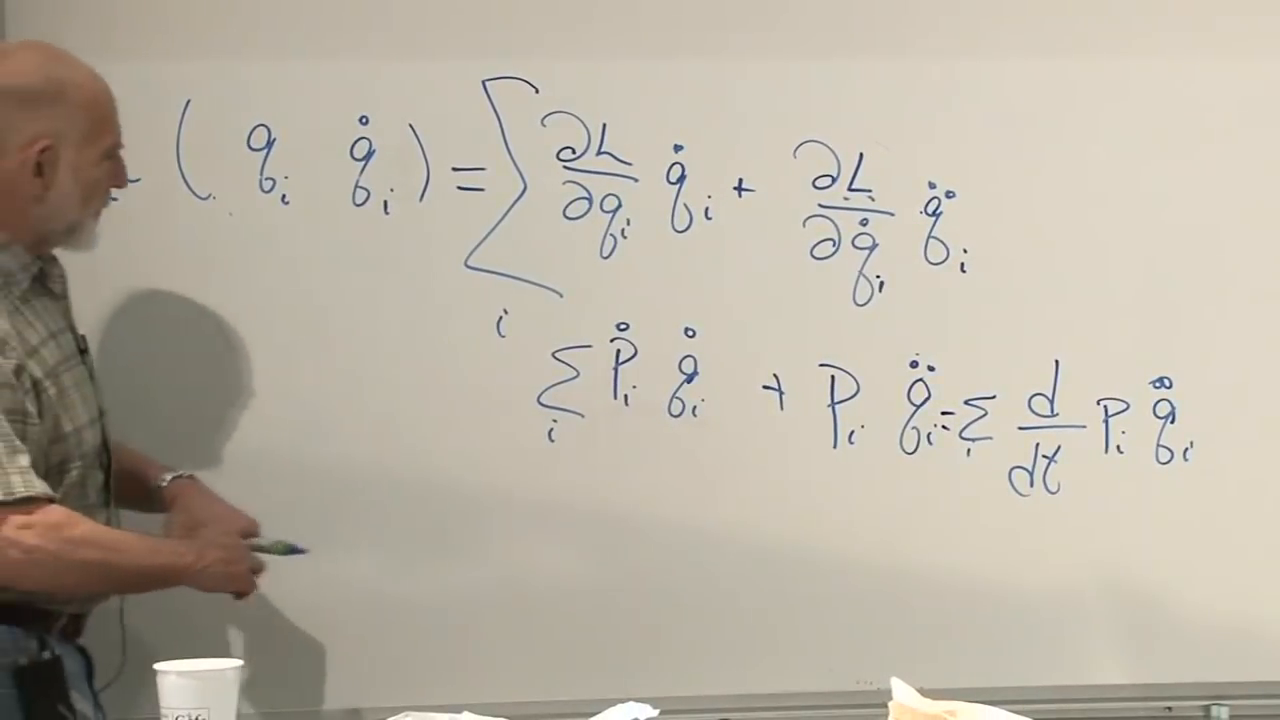
\includegraphics[width=0.84\textwidth]{lecture_05_figure_21.png}
  \caption{链式法则利用运动方程转化成了 \(\sum_i p_i\dot q_i\) 的导数。}
  \lectureframe{01:13:45}
\end{figure}

\begin{classroomqa}
  \audiencequestion{乘积中最后的 \(q_i\) 应该带一个点还是两个点？
  \lecturetimestamp{01:14:31--01:15:32}}
  \lecturerresponse{在乘积内部它是 \(p_i\dot q_i\)，带一个点。对乘积求导得到
  \(\dot p_i\dot q_i+p_i\ddot q_i\)，这解释了展开后的第二项中的两个点。}
\end{classroomqa}

将这两个导数相减，得到一个守恒组合。历史惯例选择它的负值，并称之为哈密顿量：
\begin{equation}
  H=\sum_i p_i\dot q_i-L.
  \label{eq:l5-hamiltonian-definition}
\end{equation}

\begin{figure}[htbp]
  \centering
  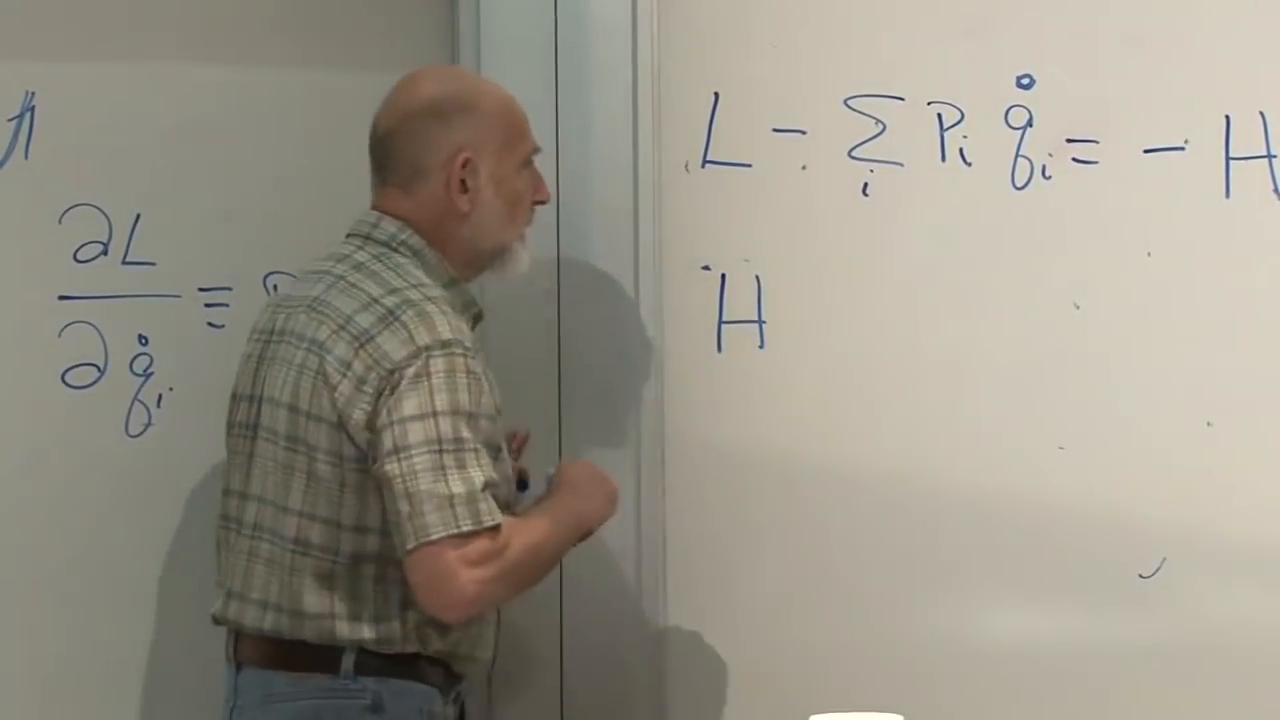
\includegraphics[width=0.80\textwidth]{lecture_05_figure_22.png}
  \caption{守恒组合 \(L-\sum_i p_i\dot q_i=-H\) 以及哈密顿量的定义。}
  \lectureframe{01:18:05}
\end{figure}

对于势场中的一个粒子，
\begin{equation}
  L=\frac12m\dot x^2-V(x),
  \qquad p=m\dot x.
  \label{eq:l5-particle-lagrangian}
\end{equation}
因此
\begin{align}
  H&=p\dot x-L
  \notag\\
   &=m\dot x^2-\left(\frac12m\dot x^2-V(x)\right)
  \notag\\
   &=\frac12m\dot x^2+V(x)=T+V.
  \label{eq:l5-particle-energy}
\end{align}

\begin{figure}[htbp]
  \centering
  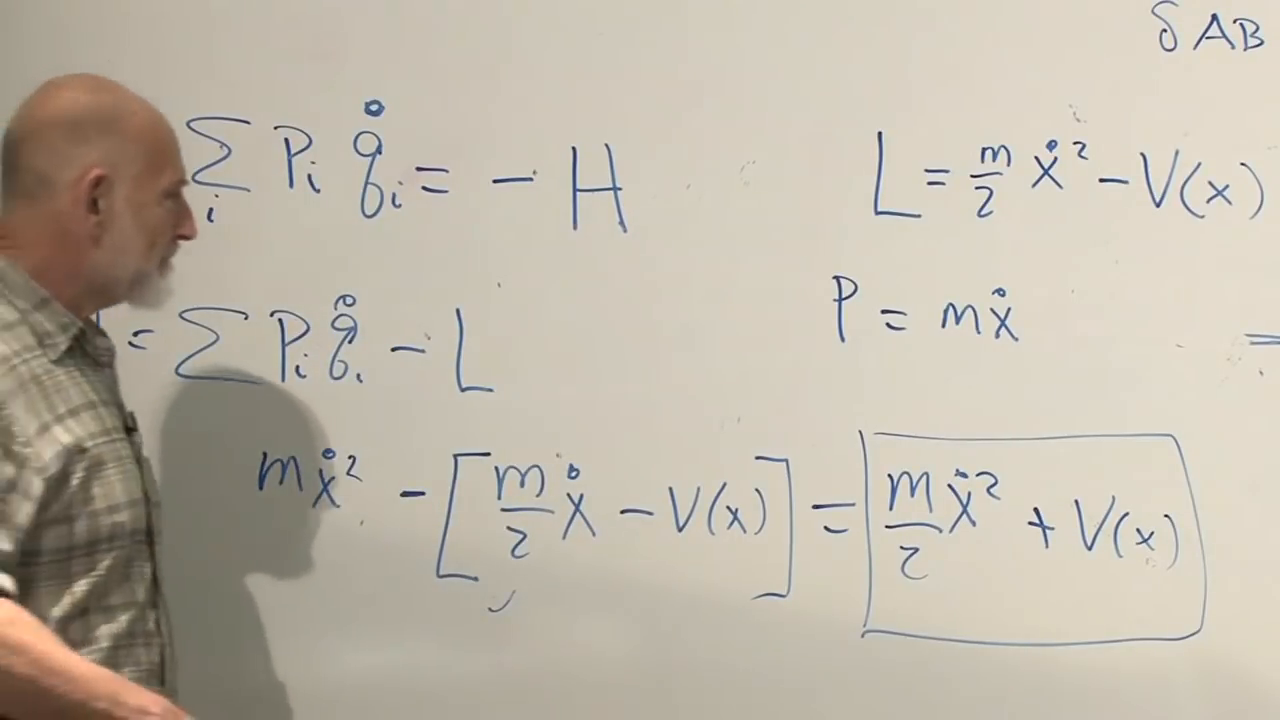
\includegraphics[width=0.86\textwidth]{lecture_05_figure_23.png}
  \caption{势场中粒子的哈密顿量化为熟悉的动能加势能。}
  \lectureframe{01:20:50}
\end{figure}

推导并未假设 \(L\) 的特定形式。因此，在这个形式体系中，式~\eqref{eq:l5-hamiltonian-definition}，而不是 \(T+V\)，才是能量的一般定义。

\section{显式时间依赖与能量交换}

在链式法则中恢复显式时间依赖：
\begin{equation}
  \frac{dL}{dt}
  =\sum_i\left(
    \frac{\partial L}{\partial q_i}\dot q_i
    +\frac{\partial L}{\partial\dot q_i}\ddot q_i
  \right)
  +\frac{\partial L}{\partial t}.
  \label{eq:l5-full-chain-rule}
\end{equation}
左边是沿运动的总导数。最后的偏导数保持 \(q\) 和 \(\dot q\) 固定，只对外部变化的参数求导。重复同样的乘积法则步骤得到
\begin{equation}
  \boxed{\frac{dH}{dt}=-\frac{\partial L}{\partial t}}.
  \label{eq:l5-hamiltonian-time}
\end{equation}

\begin{figure}[htbp]
  \centering
  \includegraphics[width=0.70\textwidth]{lecture_05_figure_04.png}
  \caption{哈密顿量仅通过拉格朗日量的显式时间依赖而变化。}
  \lectureframe{01:37:22}
\end{figure}

对于式~\eqref{eq:l5-driven-oscillator}的受驱振子，
\begin{equation}
  \frac{\partial L}{\partial t}
  =-\frac12\dot k(t)x^2,
  \qquad
  \dot H=\frac12\dot k(t)x^2.
  \label{eq:l5-driven-energy-rate}
\end{equation}
在\(x=0\)处瞬时速率消失；远离原点时，改变弹簧常数做功的速率正比于\(x^2\dot k\)。

\begin{classroomqa}
  \audiencequestion{如果能量不守恒，它的定义是哈密顿量的时间导数吗？
  \lecturetimestamp{01:27:11--01:28:04}}
  \lecturerresponse{不是。能量是\(H\)。它的导数告诉我们该能量如何变化。当拉格朗日量具有熟悉的形式时，\(H=T+V\)；当它不具有时，式~\eqref{eq:l5-hamiltonian-definition}给出定义。将系统扩大以包含外部驱动器，就恢复了总哈密顿量的守恒。}
\end{classroomqa}

\begin{classroomqa}
  \audiencequestion{这如何适用于之前旋转旋转木马上的观察者，其中出现了离心项和科里奥利项？
  \lecturetimestamp{01:28:08--01:29:52}}
  \lecturerresponse{匀速旋转的坐标系是依赖于时间的变量变换，而不是固定的空间对称性，也不是简单的时间平移。其变换后的拉格朗日量可用于构造哈密顿量，但这一单独的计算最好推迟到讨论磁力时进行，因为其代数形式密切相关。}
\end{classroomqa}

\section{拉格朗日工具箱一览}

整个结构现在可以写成一个紧凑的堆叠：
\begin{align}
  L&=L(q_i,\dot q_i,t),
  \notag\\
  p_i&=\frac{\partial L}{\partial\dot q_i},
  \qquad
  \dot p_i=\frac{\partial L}{\partial q_i},
  \notag\\
  \delta q_i&=\epsilon f_i(q)
  \quad\Longrightarrow\quad
  Q=\sum_i p_i f_i(q),\quad \dot Q=0,
  \notag\\
  H&=\sum_i p_i\dot q_i-L,
  \qquad
  \dot H=-\frac{\partial L}{\partial t}.
  \label{eq:l5-toolkit}
\end{align}

\begin{figure}[htbp]
  \centering
  \includegraphics[width=0.66\textwidth]{lecture_05_figure_03.png}
  \caption{板书回顾从\(L(q,\dot q,t)\)、正则动量以及欧拉--拉格朗日方程开始。}
  \lectureframe{01:31:37}
\end{figure}

这些公式包含一个定义、运动方程、普通连续对称性的荷以及时间平移的荷。技巧不多；重要的是能够重新推导它们，而不是记住互不相关的表达式。

\section{为什么要使用拉格朗日力学或哈密顿力学？}

\begin{classroomqa}
  \audiencequestion{力学能否同样地用\(L\)或\(H\)来描述，为什么要选择其中一种表述？
  \lecturetimestamp{01:37:16--01:39:18}}
  \lecturerresponse{当勒让德变换是正则的时，它们是等价的，但它们强调不同的结构。拉格朗日力学自然地始于驻定作用量。哈密顿力学起初更为抽象，但其方程简单，并且在量子力学中变得核心。哈密顿量是能量，但其作用远不止守恒定律。}
\end{classroomqa}

\begin{classroomqa}
  \audiencequestion{牛顿知道能量守恒的哈密顿形式吗？
  \lecturetimestamp{01:39:29--01:39:56}}
  \lecturerresponse{就历史记录所表明的而言，并非以这种表述。牛顿所陈述的框架是力定律\(F=ma\)。}
\end{classroomqa}

\begin{classroomqa}
  \audiencequestion{为什么每个物理系统都应具有拉格朗日量？这仅仅是实验性的吗？
  \lecturetimestamp{01:39:57--01:42:37}}
  \lecturerresponse{对于所考虑的封闭系统，这是一个经验事实，也源自更深层的量子描述。可以发明数学上自洽的微分方程，它们不是欧拉--拉格朗日方程。例如，\(\dot x=-x\)是完全可解的，但作为基本的封闭单坐标定律，它具有耗散那种丢失信息的特征。经典力学在逻辑上并不先于量子力学；其基本结构继承自量子力学。详细原因尚待后述。}
\end{classroomqa}

\begin{classroomqa}
  \audiencequestion{如果每个真实的封闭系统都有拉格朗日量，那么我们称为拉格朗日量的每个函数都对应于自然界中发现的系统吗？
  \lecturetimestamp{01:42:39--01:42:54}}
  \lecturerresponse{不是。形式演算允许许多函数，它们并不由任何已知物理系统实现。}
\end{classroomqa}

\begin{classroomqa}
  \audiencequestion{拉格朗日量主要是发明势的工具吗？
  \lecturetimestamp{01:42:54--01:43:32}}
  \lecturerresponse{它比这更广泛。它可以组织候选力学系统，并且常常是通向运动方程的最短实用途径。}
\end{classroomqa}

双摆展示了这一实用优势。选择两个角度，用这些角度及其时间导数计算两个质量的速度，构造\(T-V\)，并让欧拉--拉格朗日方程隐式地处理约束力。这比用\(F=ma\)分解所有张力和加速度要干净得多。

\begin{figure}[htbp]
  \centering
  \includegraphics[width=0.84\textwidth]{lecture_05_figure_05.png}
  \caption{能量速率恒等式仍留在黑板上，位于双摆草图旁边。}
  \lectureframe{01:45:39}
\end{figure}

\begin{figure}[htbp]
  \centering
  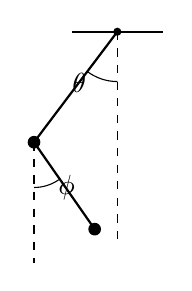
\begin{tikzpicture}[scale=1.15]
    \draw[thick] (-0.5,0) -- (0.5,0);
    \fill (0,0) circle (0.045);
    \draw[dashed] (0,0) -- (0,-2.3);
    \draw[thick] (0,0) -- (-0.92,-1.22);
    \fill (-0.92,-1.22) circle (0.07);
    \draw[dashed] (-0.92,-1.22) -- (-0.92,-2.55);
    \draw[thick] (-0.92,-1.22) -- (-0.25,-2.18);
    \fill (-0.25,-2.18) circle (0.07);
    \draw (0,-0.55) arc (-90:-127:0.55);
    \node at (-0.42,-0.56) {$\theta$};
    \draw (-0.92,-1.72) arc (-90:-55:0.48);
    \node at (-0.56,-1.72) {$\phi$};
  \end{tikzpicture}
  \caption{双摆的广义角坐标。}
\end{figure}

变量替换同样高效：先变换一个拉格朗日量，再推导其方程，而不是分别变换每一个力方程。

\begin{classroomqa}
  \audiencequestion{双摆本质上是不是另一个三体系统，比如太阳、地球和月球，其中把一个物体当作固定锚点？
  \lecturetimestamp{01:45:06--01:45:25}}
  \lecturerresponse{这个类比抓住了层级关系，尽管杆施加了不同的约束。在两种情况下，一个质量极大或固定的组成部分都可以在近似中被当作参考结构。}
\end{classroomqa}

\begin{classroomqa}
  \audiencequestion{双摆使用的是\(T-V\)，尽管刚才强调了更一般的拉格朗日量。那么\(T-V\)在什么时候成立？
  \lecturetimestamp{01:46:08--01:46:58}}
  \lecturerresponse{对于在惯性系中观察的普通非相对论粒子，且没有磁速度耦合时，这个熟悉的形式适用。旋转参考系、相对论系统以及磁场则需要更一般的项。}
\end{classroomqa}

\begin{classroomqa}
  \audiencequestion{碰撞是否不属于这一描述？
  \lecturetimestamp{01:47:00--01:48:05}}
  \lecturerresponse{弹性碰撞源于短程力，因此也源于势。非弹性碰撞在微观层面上仍然是力学的，但能量进入了内部振动、形变和热。忽略这些自由度的质心描述是不完整的。}
\end{classroomqa}

\begin{classroomqa}
  \audiencequestion{被球棒击中的棒球能否用\(F=ma\)来分析？
  \lecturetimestamp{01:48:05--01:48:33}}
  \lecturerresponse{只能在粗略层面上。完整的说明必须追踪形变、发热、球可能受到的损伤，或许还有球棒的断裂。正是这些内部自由度使得真实的撞击比质点碰撞困难得多。}
\end{classroomqa}

\begin{classroomqa}
  \audiencequestion{那么扩展的刚体呢？
  \lecturetimestamp{01:48:34--01:49:00}}
  \lecturerresponse{刚体既可以用牛顿方法研究，也可以用写成平动和转动坐标的\(T-V\)拉格朗日量来研究。构造这个拉格朗日量是一项有用的练习。}
\end{classroomqa}

\begin{classroomqa}
  \audiencequestion{量子能量--时间不确定性关系是否意味着能量不严格守恒？
  \lecturetimestamp{01:49:01--01:49:29}}
  \lecturerresponse{不是。能量可以严格守恒。该关系说的是，要以高精度分辨能量，需要在长时间内进行观测；它并不取代守恒定律。}
\end{classroomqa}

\begin{classroomqa}
  \audiencequestion{牛顿力学和拉格朗日力学在逻辑上等价吗？
  \lecturetimestamp{01:49:36--01:50:07}}
  \lecturerresponse{在两者都适用的通常范围内，它们是等价的。然而人们可以构造出这样的拉格朗日量，其方程不像基本形式\(m\ddot x=F(x)\)。}
\end{classroomqa}

\section{一个依赖于坐标的动能项}

考虑这个刻意不熟悉的例子
\begin{equation}
  L=\frac12q^2\dot q^2-\frac12q^2.
  \label{eq:l5-nonstandard-l}
\end{equation}
它是一个有效的拉格朗日量，其动能系数依赖于坐标。也可以考虑诸如\(q\dot q\)这样的速度线性项；在这个一维例子中，该特定项是一个全导数，不会改变运动方程。

正则动量是
\begin{equation}
  p=\frac{\partial L}{\partial\dot q}=q^2\dot q,
  \label{eq:l5-nonstandard-p}
\end{equation}
所以
\begin{equation}
  \dot p=q^2\ddot q+2q\dot q^2,
  \qquad
  \frac{\partial L}{\partial q}=q\dot q^2-q.
  \label{eq:l5-nonstandard-derivatives}
\end{equation}
因此运动方程是
\begin{equation}
  q^2\ddot q+q\dot q^2=-q.
  \label{eq:l5-nonstandard-eom}
\end{equation}

\begin{figure}[htbp]
  \centering
  \includegraphics[width=0.80\textwidth]{lecture_05_figure_06.png}
  \caption{在依赖于坐标的动能例子中被求导的动量。}
  \lectureframe{01:52:32}
\end{figure}

\begin{classroomqa}
  \audiencequestion{方程可以除以\(q\)吗？
  \lecturetimestamp{01:53:22--01:53:39}}
  \lecturerresponse{只能在\(q\neq0\)处。在\(q=0\)处，动能系数和勒让德映射是退化的，因此除法会丢弃一个需要单独处理的奇点。}
\end{classroomqa}

哈密顿量是
\begin{align}
  H&=p\dot q-L
  \notag\\
   &=q^2\dot q^2-
     \left(\frac12q^2\dot q^2-\frac12q^2\right)
  \notag\\
   &=\frac12q^2\dot q^2+\frac12q^2.
  \label{eq:l5-nonstandard-h}
\end{align}

\begin{classroomqa}
  \audiencequestion{\(q^2\dot q^2/2\)还能被称为动能吗？
  \lecturetimestamp{01:54:41--01:55:07}}
  \lecturerresponse{可以。在这个已解例子中，哈密顿量再次看起来像一个正的动能项加上一个势能项。关键在于，这些形式定义在事先不假设基本常质量形式的情况下仍然成立。}
\end{classroomqa}

\section{耗散以及形式体系的更深层起源}

\begin{classroomqa}
  \audiencequestion{摩擦如何被纳入拉格朗日量？
  \lecturetimestamp{01:55:09--01:56:17}}
  \lecturerresponse{在这里所考虑的简单闭合有限自由度系统中，它不是作为一种基本力被纳入的。宏观摩擦是数量巨大的微观自由度的统计效应。那些原子仍然服从底层力学，但不追踪它们的约化描述会显示出耗散。}
\end{classroomqa}

\begin{classroomqa}
  \audiencequestion{哈密顿是如何得出他的表述的？
  \lecturetimestamp{01:56:22--01:56:37}}
  \lecturerresponse{这里没有给出历史性的推导。本课程的重要任务是理解这一表述如何运作。}
\end{classroomqa}

\begin{classroomqa}
  \audiencequestion{当拉格朗日量并不明显地表现为\(T-V\)时，是否有更一般的配方来得到它？
  \lecturetimestamp{01:56:43--01:58:54}}
  \lecturerresponse{实验、有根据的猜测、对称性原理，或者从期望的方程反推，都可以提供这个函数。问微积分本身它的输入从何而来，就像问导数的定义中\(f(x)\)从何而来一样。一旦函数被指定，微积分就告诉我们该怎么做。自然界的封闭系统为何符合这一抽象结构，这个问题由量子力学在更深的层次上回答。}
\end{classroomqa}

这一点与本课程开篇的主题相关。基本的哈密顿演化是确定性的且可逆的，其意义是轨迹不会合并，信息也不会被简单地销毁。这一性质与相空间表述之间的关系将分阶段展开。

\begin{classroomqa}
  \audiencequestion{变分法是否只是从期望的经典方程反向推导，而量子力学是否以同样的方式得到它的拉格朗日量？
  \lecturetimestamp{01:59:37--02:01:07}}
  \lecturerresponse{在初等经典构造中，确实可以选择一个作用量，使其驻定路径重现已知的方程。量子力学中的逻辑顺序不同：它自然地始于哈密顿量，并可以朝着拉格朗日描述推进。在那里哈密顿量更为直观，尽管它在经典力学中最初显得抽象。}
\end{classroomqa}

\begin{classroomqa}
  \audiencequestion{量子力学能描述摩擦吗？
  \lecturetimestamp{02:01:08--02:02:05}}
  \lecturerresponse{能，但基本的描述必须包含环境的自由度。粒子在黏性流体中运动，若不考虑流体的粒子，就无法被完整描述。摩擦是当那些自由度不被逐一追踪时涌现出来的复杂集体效应。}
\end{classroomqa}
